\documentclass[letter]{article}
\usepackage{anysize}
\usepackage[spanish]{babel}
\usepackage{graphicx}
\usepackage[utf8]{inputenx}
\usepackage{listings}
\usepackage{ulem}
\usepackage{verbatim}
\usepackage{xcolor}

\marginsize{2cm}{2cm}{2cm}{2cm} %{izq}{der}{top}{bottom}

\lstset{tabsize=2,language=java,basicstyle=\scriptsize\ttfamily,numberstyle=\scriptsize\ttfamily,numbers=left,aboveskip={1.5\baselineskip},columns=fixed,showstringspaces=false,extendedchars=true,breaklines=true,prebreak = \raisebox{0ex}[0ex][0ex]{\ensuremath{\hookleftarrow}},frame=single,showtabs=false,showspaces=false,showstringspaces=false,identifierstyle=\color[rgb]{0,0,0},keywordstyle=\color[rgb]{0,0,1},commentstyle=\color[rgb]{0,0.55,0},stringstyle=\color[rgb]{1,0,0},language=java}

% ------------- preambulo -------------

\setlength{\parindent}{0in}
\setlength{\textheight}{9in}
\setlength{\parskip}{0.25in}

\begin{document}

% ------------ portada ---------------

\thispagestyle{empty}
\begin{flushleft}
  Universidad de Chile\\Facultad de Ciencias Físicas y Matemáticas\\Departamento de Ciencias de la Computación\\[4cm]
\end{flushleft}
\begin{center}
  \huge{Aplicaciones Empresariales sobre la Plataforma Java J2EE\\[1.5cm] CC5604-1\\[0.4cm]}
  \Large{\textbf{Informe de proyecto Fase 1\\[2.5cm]}Claudio Andrés Berroeta Alegría\\[0.4cm]René Fernando Tapia Pincheira\\[2.5cm]10 de mayo de 2013}
\end{center}

%-----------indice---------------------------

\newpage
\tableofcontents

%-----------introduccion---------------------

\newpage
\section{Introducción}

En el presente informe se expone, explica y resuelve el problema de la fase 1 del proyecto del curso CC5604, el cual construye la totalidad de la capa de negocios del proyecto presentando por el FC Barcelona. Para ello se nos pide como requisito escribir el código, usando session beans y entidades, y escribir tests unitarios y tests de integración para validar la correctitud funcional de la lógica del código.

A grandes rasgos, el problema propuesto consiste en crear una aplicación web administrativa para el FC Barcelona (nuestro cliente), el cual en una primera etapa desea crear la capa de negocios de la aplicación para ordenar las distintas entidades que conforman el club: personal, socios y activos.

%-----------enunciado del problema-----------
\newpage
\section{El problema}

El problema consiste en construir una aplicación administrativa de los distintos actores del club deportivo FC Barcelona. Se nos describe como funciona actualmente el FC Barcelona y nos explican como debe funcionar la nueva aplicación del club.

El FC Barcerlona tiene personal contratado y directivos, los cuales poseen en común las siguientes características: nombre, apellido, fecha de nacimiento y nacionalidad. El personal contratado se puede clasificar en: jugadores, técnicos, doctores y fisioterapeutas. 

Los jugadores, además de pertenecer al personal, también pertenecen a los activos del club; éstos se clasifican en: arqueros, defensas, mediocampistas y delanteros. Cada jugador posee un valor base y un coeficiente de valor de mercado, el cual está dado por su posición en la cancha.

Además del personal, el club posee socios, los cuales se dividen en 2: con derecho a asiento o simpatizantes. Cada socio posee los mismos datos que el personal, pero además poseen datos de contacto que pueden ser de diverso tipo.

Tanto el personal como los socios poseen un contrato con el club, el cual tiene una fecha de inicio, una fecha de expiración y una mensualidad.

Como toda institución deportiva, el FC Barcelona posee activos provenientes de sus distintos bienes, los cuales poseen un valor económico que influye en las cuentas del club. Así como también posee pasivos los cuales se declaran como pendientes o pagados.

Además la aplicación tiene usuarios registrados, los cuales poseen un nombre de usuario (único) y una contraseña.

En cuanto al proceso de negocio, se debe proveer lo siguiente: administración de usuarios, administración de contratos, administración de personal, administración de pasivos/activos y administración de finanzas del club.


%-------- solucion --------------------------
\newpage
\section{Solución del problema}
 Para empezar el proyecto FCBarcelona, primero se escogió el modelo de programación. Sabemos que el proyecto no es de gran escala, es decir, no requiere un equipo de trabajo grande para poder desarrollar la aplicación. Por lo tanto un modelo de \textit{n capas} calzaría perfecto con la descripción del problema, ya que este modelo funciona bien tanto para proyectos pequeños como para grandes, al contrario del \textit{DDD} que va orientado a  proyectos grandes. Dadas las características del proyecto, las funcionalidades son las típicas
de un sistema administrador de entidades (mantenedores), por lo tanto, el modelo de \textit{n capas} es útil ya que no esta enfocado en el negocio, más bien en la arquitectura.

Entre las ventajas del desarrollo de \textit{n capas} podemos encontrar:
\begin{itemize}
\item{El código se escribe por capas, independientes. Esto es útil para acotar los cambios de una funcionalidad a su capa y no al resto de la aplicación.}
\item{Es altamente escalable; es decir, puede ampliarse con facilidad mientras las necesidades lo estimen conveniente.}
\item{Sus componentes son independientes, por lo que puede estar distribuidos en varios servidores (escalabilidad).}
\item{La arquitectura es reusable y podría implementarse en otros proyectos, con pequeños cambios.}
\end{itemize}

Para resolver el problema se partió de la base del modelo entidad-relación entregado junto con el enunciado, el cual permitió definir las distintas entities que nos ayudarán al resolver el problema. Estas se ubicarán en la capa de cliente de la aplicación.

Siguiendo las indicaciones del enunciando, se construyeron los distintos session beans, cada uno con su respectiva interfaz asociada. Las interfaces van ubicadas en la capa del cliente junto con las entities para exponer las funcionalidades del session bean, mientras la implementación estará en la capa de negocio. En este punto se dicidió reemplazar los  \textit{session beans} clásicos de \textit{J2EE} por objetos de negocio \textit{Service} de \textit{Spring}. Se usó el framework \textit{Spring} en vez de session beans EJB ya que \textit{Spring} provee muchas más opciones a la hora de configurar, permite definir que los métodos sean transaccionales, inyectar dependencias fuera de un ambiente J2EE (útil en los tests unitarios) y en general, provee muchas más funcionalidades, compatibles con otros módulos y librerías de \textit{Spring}. A la larga es más escalable y extensible. También podría haberse empleado diractamente JDBC y realizar consultas de forma más `manual'. Esta forma la deshechamos sin duda alguna, pues diminuye la claridad al leer el código y deberíamos reinventar mucho código. Habría quedado mal, feo, con bugs y poco extensible.

Se usó el framework ORM Hibernate por poseer una robustez conocida, comunidad de desarrollo y testeo grande y prestigio a la hora de usarse en implementaciones de proyectos de pequeña a gran envergadura. La decisión de usar \textit{Hibernate} recae en el sólo hecho que la documentación es más abundante (por ser pionero en el ámbito de mapeos objetos-relación).

\newpage
\subsection{Módulo cliente}

Esta es la sección del proyecto visible para la aplicación cliente. De esta forma podemos separar la `interfaz' de la aplicación de manera temprana. Aplicaciones pequeñas, tradicionalmente, se distribuyen en un solo módulo. Aquí hemos decidido pensar a futuro y separar el codigo de forma de preparse mejor para las próximas entregas.

\subsubsection{Entities.}

Los entities nos permiten modelar entidades de negocio que pueden ser expresados como sustantivos y que son mapeados a tablas de una base de datos del tipo relacional. En la siguiente imagen se pueden apreciar las distintas entities que se desarrollaron para el proyecto.
\begin{center}
  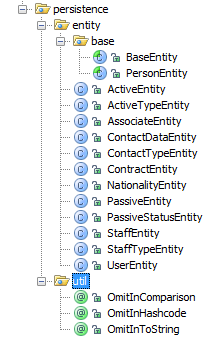
\includegraphics{images/cliente-persistence.png}
\end{center}
Un aspecto importante del proyecto es que se usó una jerarquía simple para la definición de entidades. Se utilizó BaseEntity para definir métodos comunes a todas las entidades (definición de toString, equales y hashCode). Sobre esta base, se definió PersonEntity que se usa para los socios y el personal (comparten atributos como nombre, apellido y fecha de nacimiento). En general, cada entidad hera de BaseEntity excepto AssociateEntity y StaffEntity que heredan de PersonEntity (que a su vez hereda de BaseEntity).

Cada entity hace referencia a una tabla en particular y posee métodos para setear y obtener datos de la BD. A continuación se encuentra el código de BaseEntity, en donde se usó reflexión para construir el resultado de cada método. La forma clásica o preferida es definiendo cada método en su respectiva clase, pero es poco flexible y poco tolerante a cambios en los atributos. Aquí hemos sacrificado performance (un poco), en pos de claridad y mantenibilidad del código (a la larga, código pequeño, limpio y simple es mejor).

\begin{lstlisting}
public abstract class BaseEntity implements Serializable {
           ...
	@Override public int hashCode() {...}
	@Override public boolean equals(Object yours) {...}
	@Override public String toString() {...}
}
\end{lstlisting}

A continuación hay un ejemplo de entidad, donde se muuestran los atributos, métodos y anotaciones. Hemos usado anotaciones, pues al momento de desarrollar, es más fácil, pues tenemos una visión clara de los atributos de la clase, y las columnas de la base de datos. Las demás entidades son similares.

\begin{lstlisting}
@Table(name = "USUARIO")
@Entity
public class UserEntity  extends BaseEntity {

    @OmitInComparison
    private Integer id;

    private String password;
    private String username;

    @Column(name = "ID", nullable = false, insertable = true, updatable = true, length = 10, precision = 0)
    @GeneratedValue(strategy=GenerationType.SEQUENCE, generator = "seq_USUARIO")
    @SequenceGenerator(name="seq_USUARIO", sequenceName = "seq_USUARIO")
    @Id
    public Integer getId() {return id;}
    public void setId(Integer id) {this.id = id;}

   ...
}
\end{lstlisting}

\subsubsection{Fa\c{c}ades.}

La otra parte importante del módulo cliente, es el punto de entrada a la lógica de negocio (fa\c{c}ades). La línea general del diseño de aplicaciones es usar componentes reutilizables y fácilmente intercambiables. Las implementaciones hay que pensarlas en código que no es definitivo y deben darse las facilidades para poder cambiar las implementaciones. De esta forma usamos interfaces para las componentes de negocio. No usarlas hubiese implicado acoplamiento de clases y código spaghetti. A continuación se muestran las interfaces definidas para proveer a la aplicación cliente las funcionalidades del sistema.

\begin{center}
  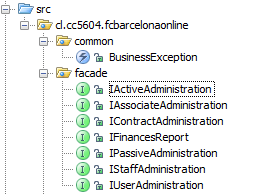
\includegraphics{images/facade.png}
\end{center}

Dado que cada funcionalidad es independiente entre sí, se distinguieron las responsabilidades y se ubicó cada una en un componente separado.

A continuación está la interfaz del administrador de usuarios. Hemos seguido la convención de llamar createX, findAllX, findById, deleteX y updateX los métodos de la lógica de negocio; de esta forma podemos crear código independiente de los gustos personales. Las demás interfaces son similares (todas proveen operaciones \textit{crud} clásicas).

\begin{lstlisting}
public interface IUserAdministration {
    void createUser(UserEntity newUser);
    List<UserEntity> findAllUsers();
    UserEntity findById(int idUser);
    UserEntity findByUsername(String username);
    void deleteUser(int idUser);
    void updateUser(UserEntity user);
}

\end{lstlisting}

Nota: una refactorización futura, en cuanto a las entidades, es remover las anotaciones de la clase y moverlas a un archivo xml separado. De esta forma evitamos exponer al cliente detalles del modelo físico de la BD. Por simplicidad, y dado que aún no se han especificado requerimientos para la aplicación cliente, hemos dejado las clases anotadas.

\newpage

\subsection{Capa de negocio.}

\subsubsection{DAO.}

La implementación de DAO usada en este proyecto corresponde a la implementación clásica de DAOs \textit{typesafe} y \textit{generic}. Se crea un DAO base genérico (usando templates y tipos paramétricos) y se especializa el DAO de cada entidad, subclaseando y proporcionando la clase de la entidad sobre la que se opera. De esta forma podemos evitar \textit{casts} innecesarios, corregir bugs de manera más efectiva y leer código de manera más fácil. Otra forma de implementarlo hubiese requerido re-definir los métodos save, delete, update, etc. en el DAO asociado a cada entidad. Esto lo descartamos pues hay mucha duplicación de código. Ahora bien, si \textit{Hibernate} provee métodos genéricos para operar con la BD, hemos usado templates para asegurarnos que los DAOs tengan responsabilidad sólo sobre una entidad particular (y no usar cualquier entidad, con cualquier dao).

Aquí la lista de los DAO que se usaron para el proyecto:

\begin{center}
  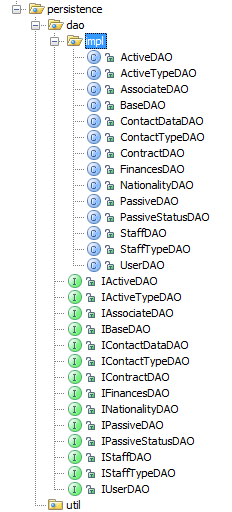
\includegraphics{images/daos.png}
\end{center}

Dado que todas las entidades requieren un conjunto común de operaciones (\textit{crud}), se ha definido un DAO base, cuya interfaz es la siguiente.

\begin{lstlisting}
public interface IBaseDAO<T, S extends Serializable> {
    List<T> findAll();
    T findById(S pk);
    void save(T object);
    void update(T object);
    void delete(T object);
    List<T> findByStatement(String statement, Object... paramPairs);
    T findOneByStatement(String statement, Object... paramPairs);
    void deleteAll();
    void flush(); 
}
\end{lstlisting}

La implementación de la interfaz anterior corresponde a operaciones genéricas en la base de datos. De esta forma, cada DAO al heredar de BaseDAO, recibe implementaciones por defecto para guardar, borrar, buscar, etc. No haber usado una interfaz común para las operaciones comunes, habría sido un error que habría costado caro en el futuro, cuando la aplicación requiera extenderse o crecer.

\begin{lstlisting}
public class BaseDAO<T, S extends Serializable> extends HibernateDaoSupport implements IBaseDAO<T, S> {

    @Autowired
    public void setFactory(SessionFactory sessionFactory) {super.setSessionFactory(sessionFactory);}

    protected Session session() {return getSessionFactory().getCurrentSession();}

    @Override
    public void flush() {session().flush();}

    @Override
    public List<T> findAll() {return (List<T>) (session().createQuery("from " + persistentClass.getSimpleName()).list());}

    @Override
    public T findById(S pk) {return (T) session().get(persistentClass, pk);}

   ...
}

\end{lstlisting}

Ahora bien, para operaciones específicas de una entidad, se agrega en su respectivo DAO (no en la base, pues no son operaciones genéricas). Podemos pensar en la capa de persistencia como 2 capas. Una capa base con operaciones genéricas y esta capa, con operaciones particulares sobre entidades. No considerar esta capa habría implicado colocar código específico de una entidad en la capa base (malo, pues el resto de DAOs lo heredarían) o colocar código de acceso a la base de datos en la lógica de negocio (más malo, pues son capas independientes, con responsabilidades distintas).
\begin{lstlisting}
public interface IUserDAO extends IBaseDAO<UserEntity, Integer> {
    public UserEntity findByUsername(String username);
}
@Repository
public class UserDAO extends BaseDAO<UserEntity, Integer> implements IUserDAO {
     ...
    @Override
    public UserEntity findByUsername(String username) {
        return findOneByStatement("from UserEntity u where u.username=:name",
                "name", username
        );
    }

}
\end{lstlisting}

\subsubsection{Capa de negocio}

La capa de negocio fue implementada en clases, anotas con \textit{@Service}. De esta forma podemos decir a \textit{Spring} que instancie automáticamente e inyecte a través de la aplicación esta instancia. La ventaja de usar\textit{Service} vs \textit{Session Beans} clásicos es la independencia del servidor de aplicaciones. Por ejemplo, al correr los tests unitarios, no es necesario levantar una instancia de servidor con \textit{Spring}; con \textit{Session Beans} sí. Además, podemos manejar transacciones anotando los métodos con \textit{@Transactional} y podemos integrar de mejor forma \textit{Hibernate} (\textit{Spring} es famoso por su facilidad a la hora de conectar componentes, además de poseer una comunidad de desarrollo activa, lo que hace difícil que quede obsoleto, por lo menos, a corto plazo). No haber usado \textit{Spring} o session beans, habría dificultado la reutilización de componentes, pues habría aglutinado el código de constructores, factories y llamadas innecesarias para inicializar objetos.

Cada componente de la capa de negocio se encarga de operar una funcionalidad particular. Por ejemplo, para la administración de usuarios, el objeto de negocio que implementa la interfaz suministrada al cliente, se encarga de la lógica de validación, y llamadas a métodos de los DAO. En caso de ocurrir algún error irrecuperable, se arroja una excepción del tipo \textit{BusinessException}, que es parte del modulo cliente. Se ha diseñado la lógica de negocio para arrojar \textit{BusinessException}s que heredan de \textit{RuntimeException}, para evitar forzar al usuario a manejar errores (con esto aportamos a la claridad del código cliente, si es que sirve de algo, claro).

A continuación mostramos parte de la implementación del administrador de usuarios:

\begin{lstlisting}
@Service
@ContextConfiguration(locations = "classpath:applicationContext.xml")
@TransactionConfiguration(transactionManager = "transactionManager", defaultRollback = false)
@Transactional(propagation = Propagation.REQUIRED, rollbackFor = {Exception.class})
public class UserAdministrationBean implements IUserAdministration {

    @Resource
    IUserDAO userDAO;

    @Override
    @Transactional
    public List<UserEntity> findAllUsers() {
        return userDAO.findAll();
    }

    @Override
    @Transactional
    public void createUser(UserEntity newUser) {
        Validator.shouldNotBeNull(newUser);
        Validator.shouldBeNull(newUser.getId());
        Validator.shouldNotBeEmpty(newUser.getUsername());
        Validator.shouldNotBeEmpty(newUser.getPassword());

        userDAO.save(newUser);
        userDAO.flush();
    }
   ...
}
\end{lstlisting}

La validación de parámetros se hace de forma directa en la lógica de negocio, pues si alguna regla no se cumple se arroja una excepción \textit{BusinessException}; además es bastante claro, las reglas de validación son reutilizables y es flexible si en el futuro se decide cambiar la lógica y validación.

\subsection{Tests}

\subsubsection{Testeo unitario y de integración}

El enfoque usado para testear los componentes difiere un poco de la forma tradicional de unit testing. Aunque se usó \textit{JUnit}, se realizan conexiones reales a una base de datos. El proyecto está configurado para cambiar rápidamente entre una base de datos \textit{Oracle} y una base de datos \textit{HSQLDB}, que permite crear bases de datos virutal en memoria (de esta forma podemos testear rápidamente sin tener que iniciar una instancia de base de datos pesada, como \textit{Oracle}).

Por un lado se han testeado los DAOs (que como sabemos, es una capa diferente a la de negocio) y comprobamos que todo marche ok a nivel de persistencia. Por otro lado se testea la capa de negocio, haciendo énfasis en las validaciones y en el resultado final del método de negocio.

Una refactorización importante futura, es quitar las dependencias entre tests, de forma que el testeo sea lo más aislado posible (unit testing como tal). En este instante, los tests de los DAOs son de integración y los de la lógica de negocio unitarios e integración (la validación es unitaria, y el resultado final es de integración, pues se conecta realmente a la base de datos para recuperar datos).

A continuación se muestra la jerarquía de tests (dependencias), en orden de ejcución que garantiza la consistencia a través de la aplicación:

\begin{center}
  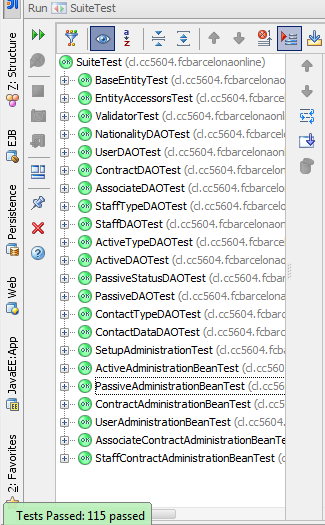
\includegraphics{images/tests.png}
\end{center}

\section{Conclusión}

Dado que se ha pedido un informe breve, no se han explicado muchos aspectos importantes. Navegando por el código se pueden apreciar las decisiones tomadas. Aunque se cuenta con poca documentación, en general, se adoptaron convenciones para nombrar variables, clases, interfaces y métodos, que corresponden a convenciones clásicas y usadas en diversos proyectos java. De esta forma es claro leer y ver el flujo de ejecución del código.

Como prototipo podemos decir que el resultado es aceptable, aunque falten muchas refactorizaciones, documentación y desacoplar algunas clases. Además, se deja abierta la posibilidad de incluir más frameworks, herramientas y dependencias como \textit{Primefaces}, \textit{Maven}/\textit{Ant} y mocks \textit{Mockito}/\textit{Easymock}.

\end{document}


